% Human computation e GWAP

\acf{HC} is a computer science technique where a computational process
performs its function by outsourcing certain steps to humans. This
\emph{outsourcing} process, as explained in the \hyperref[intro]{introduction},
is mainly due to the computational complexity of \ac{AI} algorithms. There are
some \ac{AI} problems that cannot be solved by computers or are too computational
intensive to be solved by computers in a reasonable amount of time.

Some of these are very simple tasks for humans, for example natural language
processing and object recognition are hard to solve problem for a computer,
but natural for a human being. A great example for this kind of problem
is recognizing hand-written text. Even after years of research,
humans are still faster and more accurate than computers. Other \ac{AI} problems
are too computationally expensive, such as many NP-complete problems like
Traveling Salesman problem, scheduling problems, packing problems, and FPGA
routing problems.\\

The expression \emph{\acf{HC}} in the context of computer science is already
used by \cite{cogprints499}. However is \cite{human:comp} to introduce the modern
usage of the term. It defines human computation as "\emph{a research area of
computer science that aims to build systems allowing massive collaboration between
humans and computers to solve problems that could be impossible for either to
solve alone}". A most simple and direct definition of \ac{HC} is:
\begin{quoting}\flushright
	Some problems are hard, even for the most\\
	sophisticated AI algorithms.\\
	Let humans solve it\omissis\\
	\medskip
    {\rm --- Edith Law}
\end{quoting}



\begin{figure}[htb]
    \centering
    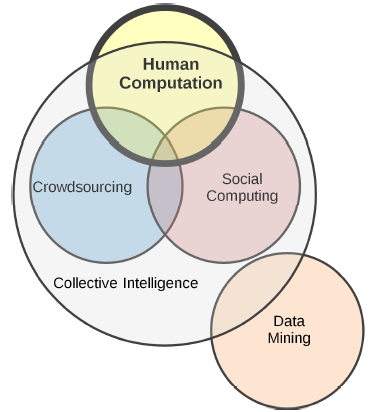
\includegraphics[width=0.6\columnwidth]{HC-relation}
    \caption{\acl{HC} relation with CrowdSourcing, Social Computing and Collective
    intelligence.}
    \label{fig:HC-relation}
\end{figure}
\acl{HC} is related with other terms, such as \emph{CrowdSourcing},
\emph{Social Computing} and \emph{Collective Intelligence} as depicted in
\autoref{fig:HC-relation}. Here we give some definitions to better understand the
similarities and the differences:
\begin{description}
    \item[CrowdSourcing] is "\emph{the act of taking a job traditionally
    performed by a designated agent (usually an employee) and outsourcing it to an
    undefined, generally large group of people in the form of an open call}"
    \cite{howe2006rise}. So it does not involve computation directly like \ac{HC}.

    \item[Social Computing] "\emph{describes any type of computing application
    in which software serves as an intermediary or a focus for a social relation}"
    \cite{schuler1994social}. So despite of the name its purpose is not computing.

    \item[Collective intelligence] defined very broadly as "\emph{groups of
    individuals doing things collectively that seem intelligent}".
\end{description}

When dealing with a human crowd the main issue is to engage users to perform tasks.
A user can be motivated to perform a task due to it's nature
(e.g. the task helps finding the cure to some disease) or to the revenue (e.g.
karma\footnote{Reputation points used in \url{www.reddit.com}.}) he/she gets for doing
such task. The most effective way for recruiting and motivating users is to give
them money\footnote{Since the ancient time. TODO ???}. For instance
\citetitle{turk} is an online tool for performing \ac{HIT} in exchange of money
rewards\footnote{The rewards for a single \ac{HIT} can be as low as 0.01\$.}.\\

\begin{figure}[htb]
    \centering
    
\includegraphics[width=\columnwidth]{HC-distribution}
    \caption{Centralized vs Distributed execution of \acl{HC}.}
    \label{fig:HC-distribution}
\end{figure}
The categorization of \ac{HC} can be further specified by adding another dimension
that involves how the tasks are executed by the users. As you can see in
\autoref{fig:HC-distribution} there are two main types of \ac{HC} execution:
\emph{centralized} and \emph{distributed}.






\subsubsection{Centralized}
In the \emph{centralized} execution we have a central hub (i.e. a website) where
users must go to perform the task. Typically the execution of a task does not
involve the offload of code and data to the user, and there is no need of ad-hoc
softwares to run the task.\\

A good example of a \emph{centralized} \ac{HC} platform is \citetitle{turk}.
\citetitle{turk} is an online platform for executing tasks in exchange of money
rewards. The platform is divided into two sections, one for the \emph{Worker}s and
one for the \emph{Requester}s. The \textbf{Worker}s are users willing to spend
time to execute a \ac{HIT} and receive the reward, the \textbf{Requester}s are
users that publish \ac{HIT} and after getting the results pay the \emph{Worker}s.\\

The lifecycle of a \ac{HIT} is the following:
\begin{enumerate}
    \item A \emph{Requester} creates a \ac{HIT} using one of the predefined project
    instances available.

    \item Once the creation is completed the \ac{HIT} is ready to be executed by
    the \emph{Worker}s.

    \item To execute a \ac{HIT} a \emph{Worker} must visit the \citetitle{turk}
    website and choose from a list of available \ac{HIT}s the one that he/she
    wants to perform (see \autoref{fig:turk}).

    \item Once the whole \ac{HIT} is completed the \emph{Requester} checks the
    result obtained and if he/she is satisfied then proceeds with the payment.
\end{enumerate}
As one can see the whole flow of the \ac{HIT} from the creation to the payment
of the \emph{Worker}s is done within the browser.\\
\begin{figure}[htb]
    \centering
    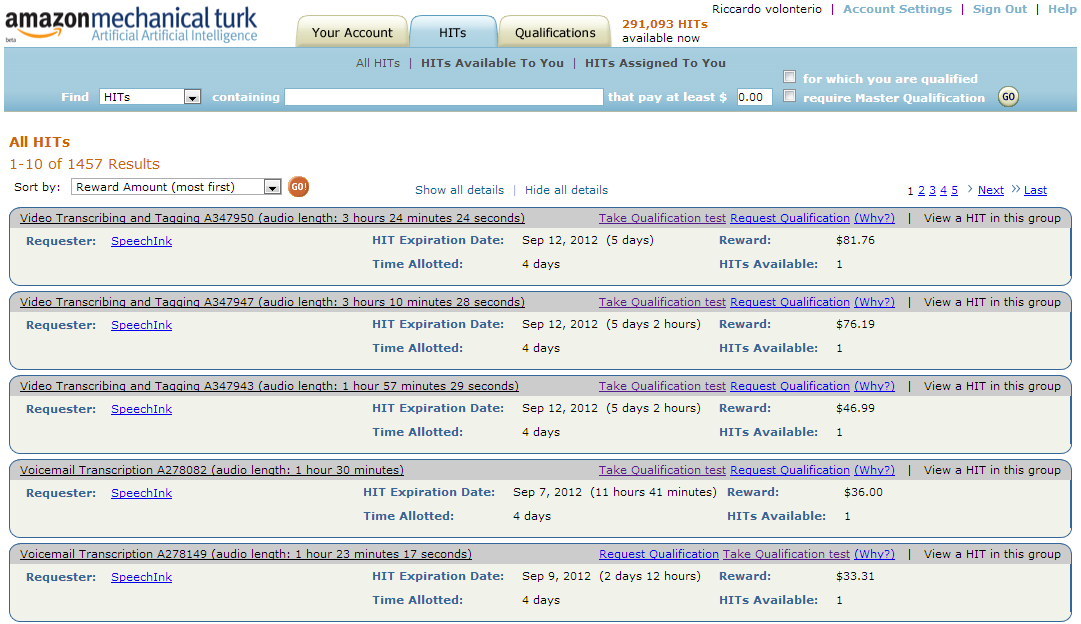
\includegraphics[width=\columnwidth]{turk}
    \caption{\citetitle{turk} web interface for choosing the \acs{HIT}.}
    \label{fig:turk}
\end{figure}


This platform has been \emph{extended} as presented in \cite{little2010turkit}
to create complete \acl{AI} algorithms able to use human computation as functions
during the execution process. The code in \autoref{lst:turkit} is an example of an
algorithm implemented using Turkit. Here \code{mturk.prompt} and \code{mturk.vote}
are \acl{HIT} executed on the \citetitle{turk} platform.
\begin{lstlisting}[language=C++,caption={Example of a Turkit algorithm.},
label={lst:turkit}]
ideas = []
for (var i = 0; i < 5; i++) {
	idea = mturk.prompt("What's fun to see in New York City? Ideas so far: " + ideas.join(", "))
	ideas.push(idea)
}
ideas.sort(function (a, b) {
	v = mturk.vote("Which is better?", [a, b])
	return v == a ? -1 : 1
})
\end{lstlisting}







\subsubsection{Distributed}
In a \emph{distributed} execution environment the central hub acts as a distribution
node in charge of offloading the task upon user request. The user can now run the
task locally without the intervention of the central hub. Eventually, when the task
is done, the user contacts the hub to upload the results.
The process of requesting the task to the hub, executing the task and sending the
results, is all done by the users, typically by a standalone piece of software
installed by the user.

% TODO ??
This solution needs the creation of ad-hoc softwares able to run on every platform
to give users an usable tool for their purpose.\\


\begin{figure}[htb]
    \centering
    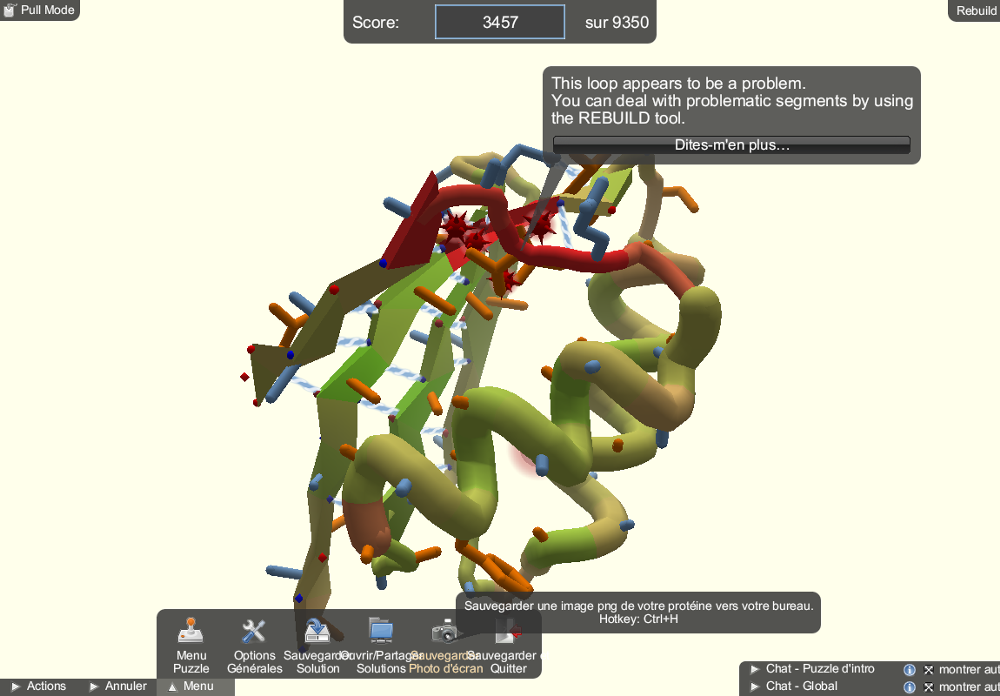
\includegraphics[width=\columnwidth]{foldit}
    \caption{The FoldIt user interface for .}
    \label{fig:foldit}
\end{figure}
An example for this kind of code distribution is the \citetitle{foldit} game.
\citetitle{foldit} is a puzzle game about protein folding, developed
by the University of Washington's Center for Game Science in collaboration with
the UW Department of Biochemistry. The objective of the game is to fold the
structure of selected proteins to the best of the player's ability. The highest
scoring solutions are analyzed by researchers, that can determine whether or not
there is a native structural configuration that can be applied to the relevant
proteins (see \autoref{fig:foldit}).







\subsubsection{\acl{GWAP}}
\acf{GWAP} is "\emph{a human-based computation technique in which a computational
process performs its function by outsourcing certain steps to humans in an
entertaining way}" von Ahn.
\ac{GWAP} come from a simple observation of data on how many hours are spent
playing games. \cite{von2008designing} reported that, accordingly to the
Entertainment Software Association\footnote{Game data from
\url{www.theesa.com/facts/gamer_data.php}}, more than 200 million hours are spent
each day playing computer and video games in the U.S.. Indeed, by age 21, the
average American has spent more than 10,000 hours playing such games equivalent
to five years of working a full-time job 40 hours per week.\\

The simple idea behind \ac{GWAP} is \emph{why not make playing games useful}?
If a task can be transformed into a game the user can be motivated to play the
game so there is no need of other types of reward (i.e. money) for doing such
task. The entertainment of playing the game itself can be used as a reward for
the user.\\

The ESP game, is a \ac{GWAP} developed by Luis von Ahn to perform image tagging.
The users' task is to agree on a word that would be an appropriate label for the
recognition of the image as described in \cite{von2004labeling}. Another \ac{GWAP}
by von Ahn is Peekaboom, where users help computers locating objects in images.